\documentclass[11pt, a4paper]{article}
\usepackage[a4paper, margin=1in]{geometry}

\usepackage{adjustbox}
\usepackage{mathtools}
\usepackage{amsmath}
\usepackage{amssymb}
\usepackage{amsthm}

\usepackage{pgfplots}
\usepackage{pst-func, pstricks-add}
\usepackage{listings}
\usepackage{color}
\usepackage{tikz}

\usepackage{textcomp}
\usepackage{soul}

\usepackage[hidelinks]{hyperref}
\pgfplotsset{width=7.5cm,compat=1.12}
\usepgfplotslibrary{fillbetween}
\pgfplotsset{compat=1.8}
\usepgfplotslibrary{statistics}
\usepackage[makeroom]{cancel}
\title{\bf{Homework \textnumero 11}}
\author{Author: David Oniani
\\
\ \ \ Instructor: Dr. Eric Westlund}
\date{March 17, 2019}

\usepackage{listings}
\usepackage{color}

%%%%%%%%%%%%%%% S E T S %%%%%%%%%%%%%%%
\newcommand{\nats}{\mathbb{N}}
\newcommand{\ints}{\mathbb{Z}}
\newcommand{\rats}{\mathbb{Q}}
\newcommand{\reals}{\mathbb{R}}
\newcommand{\irrats}{\mathbb{I}}

\newcommand{\pnats}{\mathbb{N}^+}
\newcommand{\pints}{\mathbb{Z}^+}
\newcommand{\prats}{\mathbb{Q}^+}
\newcommand{\preals}{\mathbb{R}^+}
\newcommand{\nreals}{\mathbb{R}^-}

\newcommand{\nints}{\mathbb{Z}^-}
\newcommand{\nrats}{\mathbb{Q}^-}
%%%%%%%%%%%%%%%%%%%%%%%%%%%%%%%%%%%%%%%

% Calligraphy
\newcommand\und[1]{\underline{\smash{#1}}}

% Operators
\DeclarePairedDelimiter\abs{\lvert}{\rvert}
\DeclarePairedDelimiter\ceil{\lceil}{\rceil}
\DeclarePairedDelimiter\floor{\lfloor}{\rfloor}

% Other
\newcommand{\rarr}{\rightarrow}

\definecolor{dkgreen}{rgb}{0,0.6,0}
\definecolor{gray}{rgb}{0.5,0.5,0.5}
\definecolor{mauve}{rgb}{0.58,0,0.82}
\definecolor{backcolour}{rgb}{0.95,0.95,0.92}

\lstset{
backgroundcolor=\color{backcolour},
aboveskip=3mm,
belowskip=3mm,
showstringspaces=false,
columns=flexible,
basicstyle={\small\ttfamily},
numbers=left,
numberstyle=\normalsize\color{gray},
keywordstyle=\color{blue},
commentstyle=\color{dkgreen},
stringstyle=\color{mauve},
breaklines=true,
breakatwhitespace=true,
tabsize=4
}


\begin{document}
\maketitle
\begin{itemize}
\item[16.1]
\begin{itemize}
\item[(a)]
The standard deviation is $\dfrac{\sigma}{\sqrt{n}} = \dfrac{125}{\sqrt{170100}} \approx 0.3031$.

\item[]

\item[(b)]
According to the 95 part of the 68-95-99.7 rule, 95\% of all values
of $\overline{x}$ fall within 2 standard deviations on either side of the unknown
mean $\mu$. Therefore, 2 is the missing number. Or in other words, 2 standard deviations
which numerically is $2 \times 0.3031 = 0.6062$.

\item[]

\item[(c)]
It is (285 - 0.6062, 285 + 0.6062) which is (284.3938, 285.6062).
Or in other words, the confidence interval is between 284.3938 and 285.6062.
\end{itemize}

\item[]
\item[]

\item[16.2]
\begin{itemize}
\item[(a)]
For 95\%, we know that the $z^*$ value is 1.960.\\\\
Therefore, the confidence interval is $(12 - 1.960 \times \dfrac{42}{400}, 12 + 1.960 \times \dfrac{42}{400})$
which is $(7.884, 16.116)$. Or in other words, the confidence interval
is between 7.884 and 16.116.

\item[]

\item[(b)]
We are 95\% confident that the mean change in score $\mu$ in the population of all high
school seniors is greater than 0. This is because the 95\% confidence interval is completely
above 0.
\end{itemize}

\item[]
\item[]

\item[16.4]
\begin{itemize}
\item[(a)]
The confidence interval is (0.51 - 0.04, 0.51 + 0.04) which is (0.47, 0.55).
Or in other words, the confidence interval is between 0.47 and 0.55.

\item[]

\item[(b)]
In 95\% of all possible samples of the same sample size, the confidence interval
will contain the true value of the population parameter.
\end{itemize}

\newpage

\item[16.5]
We need to look the $z$-score for the value $\dfrac{1 - 0.75}{2} = 0.125$.
From Table A, we get that $z = -1.15$. Now, we flip the sign and get that
$z^* = 1.15$. Below is the sketch.
\item[]
\item[]
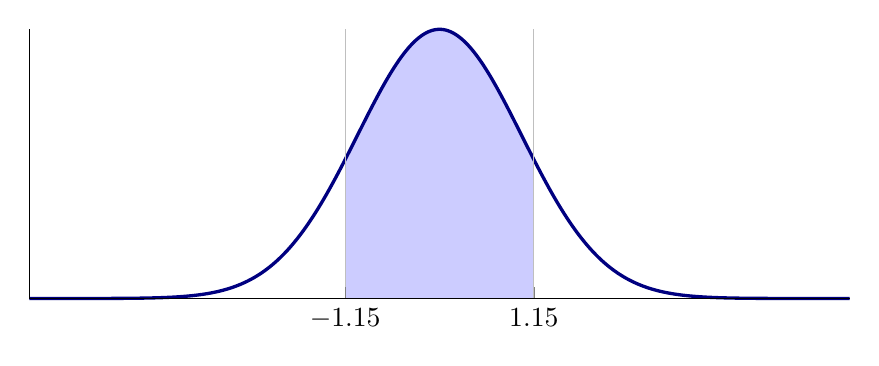
\begin{tikzpicture}
    \pgfmathdeclarefunction{gauss}{2}{%
    \pgfmathparse{1/(#2*sqrt(2*pi))*exp(-((x-#1)^2)/(2*#2^2))}%
    }
    \begin{axis}[
      no markers, domain=-5:5, samples=1000,
      axis lines*=left,
      every axis y label/.style={at=(current axis.above origin),anchor=south},
      every axis x label/.style={at=(current axis.right of origin),anchor=west},
      height=5cm, width=12cm,
      xtick={-1.15, 1.15}, ytick=\empty,
      enlargelimits=false, clip=false, axis on top,
      grid = major
      ]
      \addplot [fill=blue!20, draw=none, domain=-1.15:1.15] {gauss(0,1)} \closedcycle;
      \addplot [very thick,blue!50!black] {gauss(0,1)};
    \end{axis}
\end{tikzpicture}

\item[]
\item[]

\item[16.7]
\begin{quote}
\begin{itemize}
\item[(a)]
Below is the stemplot for the data.
\item[]
\begin{tabular}{r | *{120}{c}}
    7 & 2 & 4\\
    8 & 6 & 9\\
    9 & 1 & 3 & 6 & 8\\
    10 & 0 & 2 & 3 & 3 & 3 & 4 & 5 & 7 & 8\\
    11 & 1 & 1 & 2 & 2 & 2 & 4 & 4 & 4 & 8 & 9\\
    12 & 0 & 8\\
    13 & 0 & 2
\end{tabular}
\item[]
\item[]
The stemplot shows two relatively low scores 72 and 74.
Other than these two, there seem to be no outliers
and no other deviations from the normality of the distribution.


\item[]

\item[(b)]
\und{\textbf{PLAN}}\\\\
We will estimate $\mu$ using the 99\% confidence interval.\\\\

\und{\textbf{SOLVE}}\\\\
$\overline{x} = \dfrac{114 + 100 + \dots + 112 + 93}{31} \approx 105.84$.
Then, the $z^*$ for 99\% is 2.576. Finally, we have that the confidence
interval is (105.84 - 2.576$\times \dfrac{15}{\sqrt{31}}$, 105.84 + 2.576$\times \dfrac{15}{\sqrt{31}}$) which is approximately
(98.90, 112.78). Or in other words, the confidence interval for $\mu$ is between 98.90 and 112.78.\\\\

\und{\textbf{SOLVE}}\\\\
We are 99\% certain that the mean IQ of seventh-grade girls is between
98.90 and 112.78.
\end{itemize}
\end{quote}

\newpage

\item[16.10]
\begin{itemize}
\item[(a)]
Using Table C, we find the $z^*$ value which is 1.645.
Then the confidence interval is between $12 - 1.645 \times \dfrac{42}{\sqrt{400}} \approx 8.55$
and $12 + 1.645 \times \dfrac{42}{\sqrt{400}} \approx 15.45$. Finally,
the confidence interval is (8.55, 15.45) or in other words, it is between
8.55 and 15.45.

\item[]

\item[(b)]
The margin of error is $1.645 \times \dfrac{42}{\sqrt{400}} \approx 3.45$.
As the confidence level decreases, the certainty that the confidence interval
will contain the true value of the population mean also decreases. This means
that the margin of error decreases.

\item[]

\item[(c)]
For 95\%, the $z*$ is 1.960. Then the margin of error is $1.96 \times \dfrac{42}{\sqrt{100}} \approx 8.23$.

\item[]

\item[(d)]
Margin of error will increase.
\end{itemize}

\item[]
\item[]

\item[16.19]
\begin{itemize}
\item[(a)]
For 99\%, the $z^*$ is 2.576. Then the confidence interval
is ($15.3 - 2.576 \times \dfrac{8.5}{\sqrt{464}} \approx 15.3$, $15.3 + 2.576 \times \dfrac{8.5}{\sqrt{464 }} \approx 15.3$)
which is, approximately, the confidence interval (14.28, 16.31). Or in other words,
the confidence interval is between 14.28 and 16.31.

\item[]

\item[(b)]
These 463 students of the class must be a random
sample drawn from all of the first-years.
\end{itemize}

\item[]
\item[]

\item[16.21]
In this case, the margin of error is $2.576 \times \dfrac{8.5}{\sqrt{464}} \approx 1.02$.
The confidence interval is therefore (36.8 - 1.02, 36.8 + 1.02) which is (35.78, 37.82).
Or in other words the confidence interval is between 35.78 and 37.82.
The new interval seems to be of the same size, yet it is shifted to the right.
The conclusion is that outliers can greatly change some results (mean, standard deviation etc.),
but they usually do not have a big impact on the margin of error (notice that the margin
of error was same in the exercise 16.19 and was $2.576 \times \dfrac{8.5}{\sqrt{464}} \approx 1.02$).

\item[]
\item[]

\item[16.22]
The student is not right. The 95\% implies that 95\% of the experiments
will include the true mean, but 5\% will not.

\item[]
\item[]

\item[16.23]
The student is not right. Future samples have no memory of what happened before.
The right way to state it would be to say: if we repeated the sample over and over,
95\% of all future sample means would be within 1.96 standard deviations of the true mean.
Once again, future samples will have no memory of this sample.
\end{itemize}

\end{document}
